\vspace{10pt}

{\centering\subsection*{郭睿:《小狗钱钱》读后感}}

\addcontentsline{toc}{subsection}{郭睿:《小狗钱钱》读后感}

\renewcommand{\leftmark}{郭睿:《小狗钱钱》读后感}

\begin{figure}[htbp]

\centering

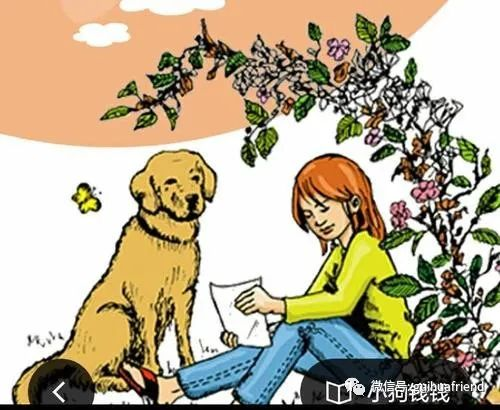
\includegraphics[width = .5\textwidth]{./ch/25.jpg}

\end{figure}



我看过很多书,这本就是其中之一,这本书写了很多关于平时的事情。

小狗钱钱,这本书让我评价,我评价是很好。这本书内容充分,主人公是吉娅和他可爱的小狗——钱钱,这本书吉娅追求三个愿望,最后三个愿都实现了,因为小狗钱钱一直鼓励吉娅,所以吉娅可以实现愿望。这本书开头写了吉娅捡到一条狗,就是钱钱,其实钱钱有他的主人,它的主人金先生出车祸住院了,钱钱没人管,就跑到吉娅门口去了。这本童话书很有趣。

这本书让我体会到了,做某件事必须要实际行动才可以成功!





\vspace{10pt}



作者:六(4)班 郭睿



指导老师:于鸿锦



投稿:2021年5月11日



发表:2021年5月13日






                



\vspace{10pt}

\hline



